% Options for packages loaded elsewhere
\PassOptionsToPackage{unicode}{hyperref}
\PassOptionsToPackage{hyphens}{url}
%
\documentclass[
]{article}
\usepackage{amsmath,amssymb}
\usepackage{lmodern}
\usepackage{ifxetex,ifluatex}
\ifnum 0\ifxetex 1\fi\ifluatex 1\fi=0 % if pdftex
  \usepackage[T1]{fontenc}
  \usepackage[utf8]{inputenc}
  \usepackage{textcomp} % provide euro and other symbols
\else % if luatex or xetex
  \usepackage{unicode-math}
  \defaultfontfeatures{Scale=MatchLowercase}
  \defaultfontfeatures[\rmfamily]{Ligatures=TeX,Scale=1}
\fi
% Use upquote if available, for straight quotes in verbatim environments
\IfFileExists{upquote.sty}{\usepackage{upquote}}{}
\IfFileExists{microtype.sty}{% use microtype if available
  \usepackage[]{microtype}
  \UseMicrotypeSet[protrusion]{basicmath} % disable protrusion for tt fonts
}{}
\makeatletter
\@ifundefined{KOMAClassName}{% if non-KOMA class
  \IfFileExists{parskip.sty}{%
    \usepackage{parskip}
  }{% else
    \setlength{\parindent}{0pt}
    \setlength{\parskip}{6pt plus 2pt minus 1pt}}
}{% if KOMA class
  \KOMAoptions{parskip=half}}
\makeatother
\usepackage{xcolor}
\IfFileExists{xurl.sty}{\usepackage{xurl}}{} % add URL line breaks if available
\IfFileExists{bookmark.sty}{\usepackage{bookmark}}{\usepackage{hyperref}}
\hypersetup{
  pdftitle={The New Governor: Facebook's Content Moderation},
  hidelinks,
  pdfcreator={LaTeX via pandoc}}
\urlstyle{same} % disable monospaced font for URLs
\usepackage[margin=1in]{geometry}
\usepackage{graphicx}
\makeatletter
\def\maxwidth{\ifdim\Gin@nat@width>\linewidth\linewidth\else\Gin@nat@width\fi}
\def\maxheight{\ifdim\Gin@nat@height>\textheight\textheight\else\Gin@nat@height\fi}
\makeatother
% Scale images if necessary, so that they will not overflow the page
% margins by default, and it is still possible to overwrite the defaults
% using explicit options in \includegraphics[width, height, ...]{}
\setkeys{Gin}{width=\maxwidth,height=\maxheight,keepaspectratio}
% Set default figure placement to htbp
\makeatletter
\def\fps@figure{htbp}
\makeatother
\setlength{\emergencystretch}{3em} % prevent overfull lines
\providecommand{\tightlist}{%
  \setlength{\itemsep}{0pt}\setlength{\parskip}{0pt}}
\setcounter{secnumdepth}{-\maxdimen} % remove section numbering
\ifluatex
  \usepackage{selnolig}  % disable illegal ligatures
\fi

\title{The New Governor: Facebook's Content Moderation}
\author{}
\date{\vspace{-2.5em}}

\begin{document}
\maketitle

\begin{itemize}
\tightlist
\item
  \protect\hyperlink{introduction}{Introduction}
\item
  \protect\hyperlink{response-to-recent-public-pressure}{Response to
  Public Pressure}
\item
  \protect\hyperlink{the-limits-of-content-moderation}{The Limits of
  Content Moderation}
\item
  \protect\hyperlink{conclusion}{Conclusion}
\item
  \protect\hyperlink{session-info}{Session info}
\end{itemize}

\hypertarget{introduction}{%
\section{Introduction}\label{introduction}}

\begin{center}\rule{0.5\linewidth}{0.5pt}\end{center}

\hypertarget{a-primer-on-content-moderation}{%
\subsubsection{A Primer on Content
Moderation}\label{a-primer-on-content-moderation}}

Facebook is one of the
\href{https://harvardlawreview.org/wp-content/uploads/2018/04/1598-1670_Online.pdf}{New
Governors}; it employs a complicated mixture of
\href{https://www.theverge.com/2020/11/13/21562596/facebook-ai-moderation}{machine
learning} and
\href{https://www.npr.org/2020/11/18/936282353/facebook-contract-workers-demand-safer-conditions-amid-pressure-to-return-to-off}{human
bureaucrats} to moderate a large segment of the world's communications
system according to their
\href{https://www.facebook.com/communitystandards/}{Community
Standards}. For better or worse, because of the First Amendment, the
work of curtailing objectionable content from our online information
ecosystem falls to private corporations like Facebook.

Recently, this governance has become a lightning rod for political
criticism. Critics from all sides of the political spectrum have
excoriated Facebook for its role in spreading
\href{https://www.npr.org/2021/03/06/974394783/far-right-misinformation-is-thriving-on-facebook-a-new-study-shows-just-how-much}{disinformation}
and \href{https://news.un.org/en/story/2020/12/1080832}{hate speech} and
\href{https://www.npr.org/2020/11/14/934833214/conservatives-flock-to-mercer-funded-parler-claim-censorship-on-facebook-and-twi}{``censoring''
conservatives}. This dissatsification has emerged most concretely in
debates surrounding amendments to
\href{https://www.businessinsider.com/what-is-section-230-internet-law-communications-decency-act-explained-2020-5}{Section
230} of the Communications Decency Act, which confers broad immunity to
technology companies from legal liability for user-generated content.

Major revisions to Section 230 would significantly change the Internet
as we know it, so policymakers must study the complex realities behind
the media narratives surrounding Facebook's content moderation before
taking action. Luckily, as part of its quarterly
\href{https://transparency.fb.com/data/}{Transparency Report}, the
company has regularly published
\href{https://transparency.fb.com/data/community-standards-enforcement}{data}
about its content moderation since 2017. Below I explain these data and
then outline a set of questions explored here.

\hypertarget{explanation-of-facebook-transparency-data}{%
\subsubsection{Explanation of Facebook Transparency
Data}\label{explanation-of-facebook-transparency-data}}

The data provide information about content moderation decisions made by
Facebook and Instagram. Specifically, they contain metrics like number
of overall ``actions'' (i.e.~deletions), proactive actions
(i.e.~deletions without human flagging), appeals, and restores with and
without appeal. These metrics are provided broken down by the 12
categories of content (enumerated
\href{https://transparency.fb.com/policies/}{here}) prohibited according
to the Community Standards. I tidied the data and broke it up into two
data frames containing the same variables: one for Facebook and one for
Instagram. Here I focus solely on data for Facebook's content moderation
due to the poor quality of published Instagram's data.

\hypertarget{questions-to-explore}{%
\subsubsection{Questions to Explore}\label{questions-to-explore}}

After an initial glimpse at the data, I have the following questions
about Facebook's content moderation:

\begin{itemize}
\item
  Has Facebook's content moderation changed in response to the recent
  wave of public attention paid to its practices?

  \begin{itemize}
  \tightlist
  \item
    If so, what types of content has the company begun to recently
    address?
  \end{itemize}
\item
  What categories of prohibited content is Facebook able to moderate
  least and most successfully?
\item
  What implications do the answers to these questions have to policy
  debates surrounding Section 230 of the Commmunications Decency Act?
\end{itemize}

\hypertarget{response-to-recent-public-pressure}{%
\subsection{Response to Recent Public
Pressure}\label{response-to-recent-public-pressure}}

\begin{center}\rule{0.5\linewidth}{0.5pt}\end{center}

Over the last few years, Facebook's content moderation has come under
increasing scrutiny everywhere from the media to electoral politics. I
hypothesize that Facebook would adapt to this increased pressure by
taking a more aggressive stance against categories of content viewed as
particularly objectionable by the public. I start my analysis with a big
picture look at the number actions Facebook has taken against
unacceptable content over the last few years:

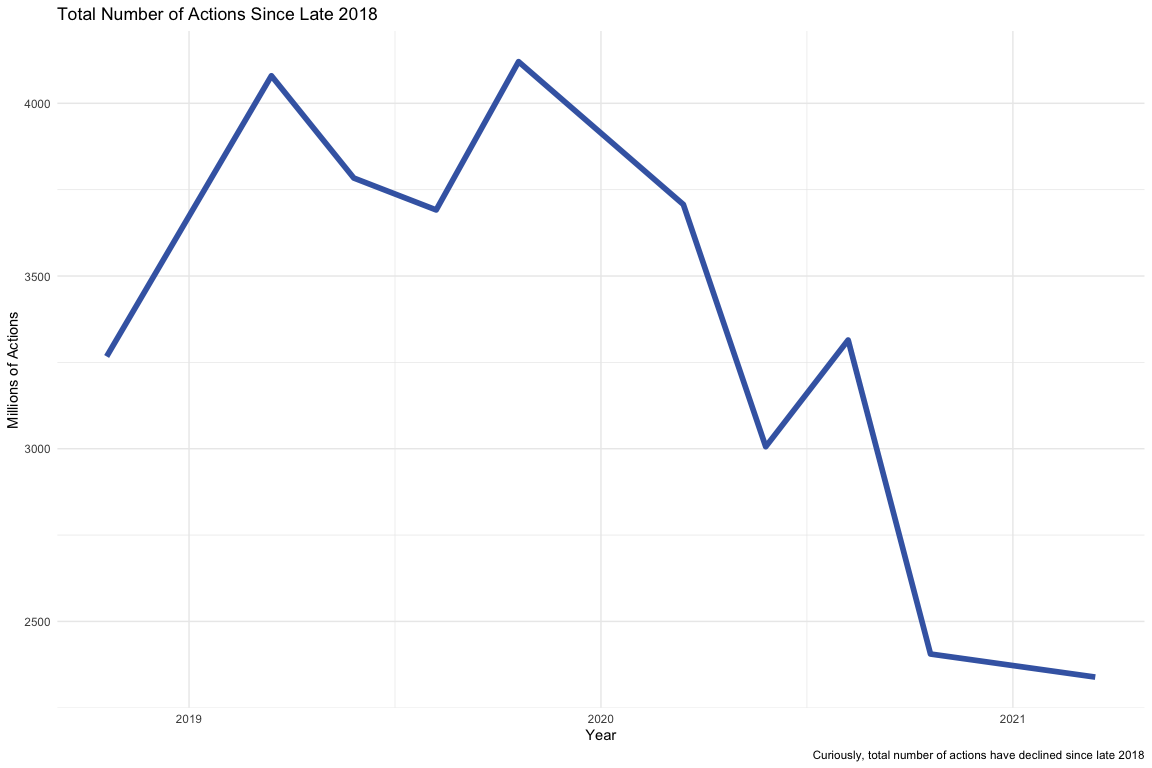
\includegraphics{pdf_document_files/figure-latex/total actions taken-1.pdf}

At first, this figure surprises. Facebook has taken \emph{fewer} actions
to moderate content since late 2018? If anything, public pressure
demands more investment and care in curtailing unacceptable content from
the social networking giant. What explains this seeming discrepancy?
Luckily, we have more information at our disposal; we break down the
total number of actions by policy area (i.e.~category of restricted
content).

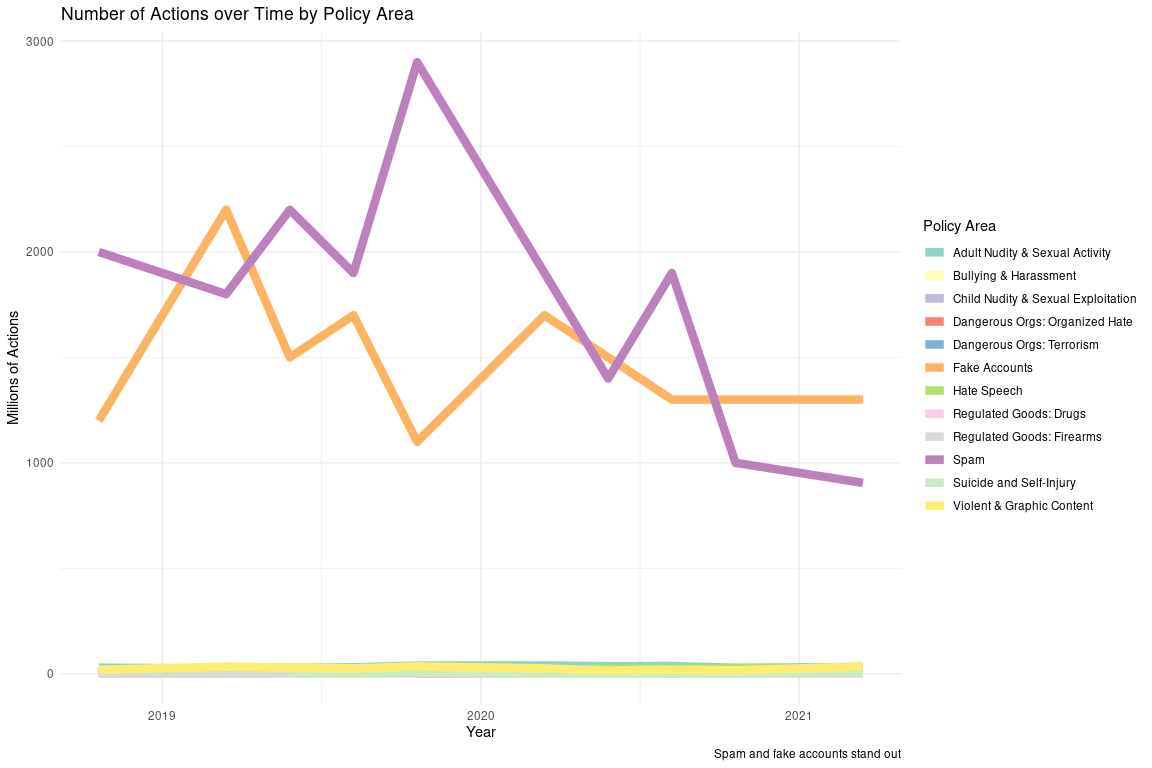
\includegraphics{pdf_document_files/figure-latex/total actions by policy area-1.pdf}

The figure above makes clear that the \emph{vast} majority of actions
taken by Facebook's content moderation system are against spam content
and fake accounts. All other categories pale in comparison to the point
that they barely register on the graph. Changes in the amount of spam
and fake content moderated will have profound effects upon the total
number of actions taken. Just to drive the magnitude of these two
categories of content home, I break down the number of actions in a
stacked bar graph:

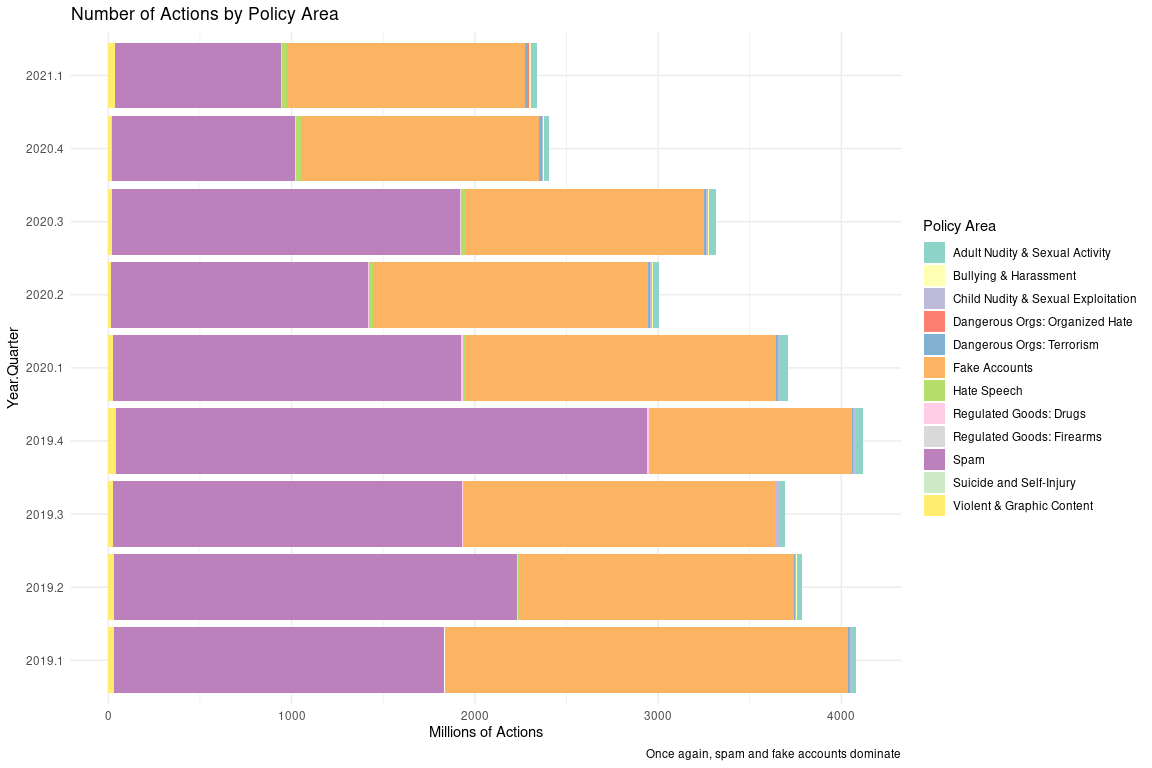
\includegraphics{pdf_document_files/figure-latex/stacked bar-1.pdf}

But we have yet to answer our initial question! Why are the total number
of actions going down in spite of recent public attention to content
moderation? It is clear from the graph above that number of actions
against spam and fake accounts are decreasing, but what about the other
categories? Perhaps their changes are more in line with our hypothesis
of greater aggressiveness in content moderation. Let us find out.

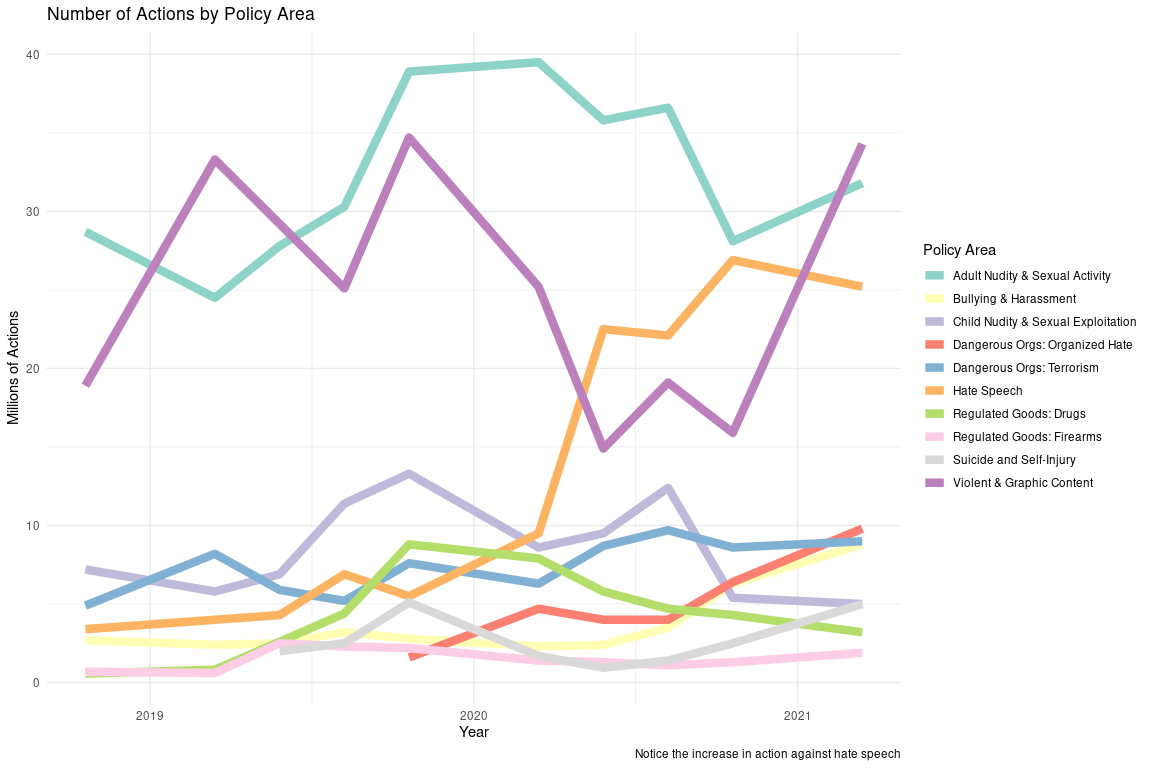
\includegraphics{pdf_document_files/figure-latex/no spam or fake accounts-1.pdf}

Once spam and fake accounts have been removed from the plot, it becomes
clear that the overall decrease is almost entirely explained by their
diminution. The other policy areas while smaller show no clear downward
trajectory. Three categories stand out in this plot for their magnitude:
Violent \& Graphic Content, Adult Nudity \& Sexual Activity, and Hate
Speech.

The latter is particularly interesting as its increase during 2020 might
reflect greater attention by Facebook to addressing criticisms related
to hate speech on its platform. While it is possible that this increase
is due to background events, the jump in number of actions is sudden
enough that Facebook could have started more actively curtailing it in
response to public pressure. Here we have a confirmatory indicator for
our hypothesis.

\hypertarget{the-limits-of-content-moderation}{%
\subsection{The Limits of Content
Moderation}\label{the-limits-of-content-moderation}}

\begin{center}\rule{0.5\linewidth}{0.5pt}\end{center}

Like any other computational tool, the machine learning elements of
Facebook's content moderation are imperfect. It is known that machine
learning algorithms struggle to understand a content's context to the
same degree a typical human can. Some categories of content then simply
defy easy classification for machines. Therefore, I hypothesize that
categories of content which require strong reference to their context
are more error prone than categories that are easier to define in a
stricter sense.

I test this hypothesis by comparing the proactive rate and percent of
actions appeals across each category of content. Context-dependent
categories like Hate Speech and Bullying \& Harassment will be less
efficacious than more objectively definable categories like Spam and
Child Nudity \& Sexual Exploitation. That is, context-dependent
categories will have lower proactive rates and higher percentages of
appeal relative to more objective categories.

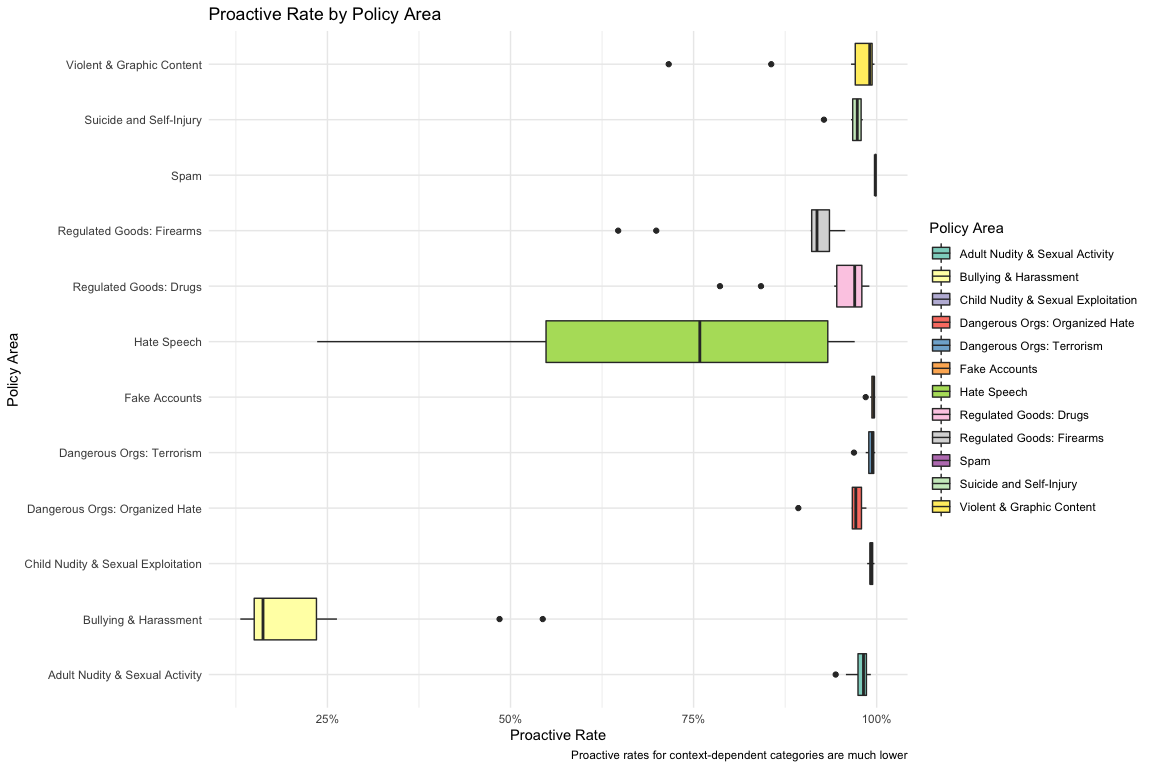
\includegraphics{pdf_document_files/figure-latex/proactive rate box plot-1.pdf}
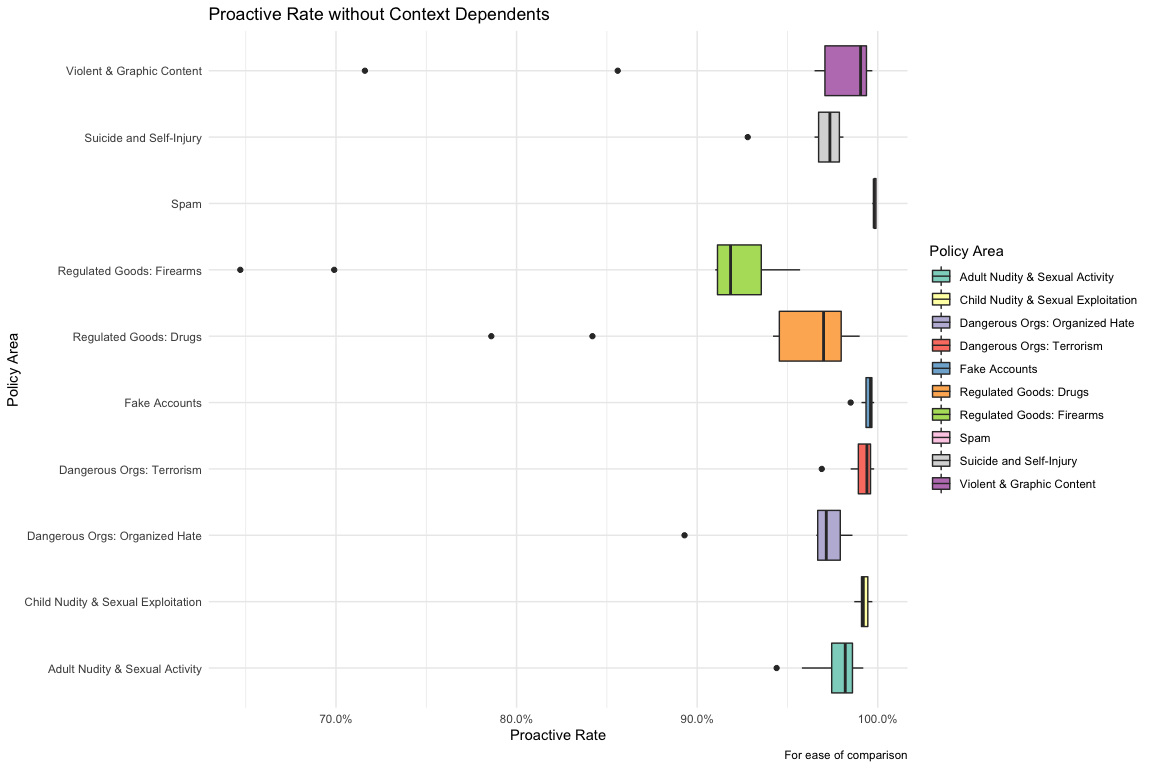
\includegraphics{pdf_document_files/figure-latex/proactive rate box plot-2.pdf}
The above graph is in line with the hypothesis. The proactive rate
measures the percentage of actioned content removed prior to any human
flags, i.e.~detected by machines without human assistance. It is thus a
measure of the efficacy of machine learning algorithms for each content
category. The box plots show the central tendency and distribution of
this rate by policy area. One can see that the context dependent groups
are both systematically lower and more variable than the more objective.

In particular, detection of Bullying \& Harassment is startlingly low
and Hate Speech unacceptably variable. In the box plot without these two
categories, it is easy to see that every other category possesses
proactive rates in excess of 90\%, especially the most objective
categories like Child Nudity \& Sexual Exploitation and Spam which are
near perfect. Machine learning algorithms are thus limited in their
capacity to deal with context-dependent content, a weakness that ensures
some user exposure.

If artificial intelligence is less likely to correctly flag
context-dependent content, what of when it does assert a classification?
Will it be prone to making disproportionate errors? I check this below
by comparing the percentage of appeals across policy areas.

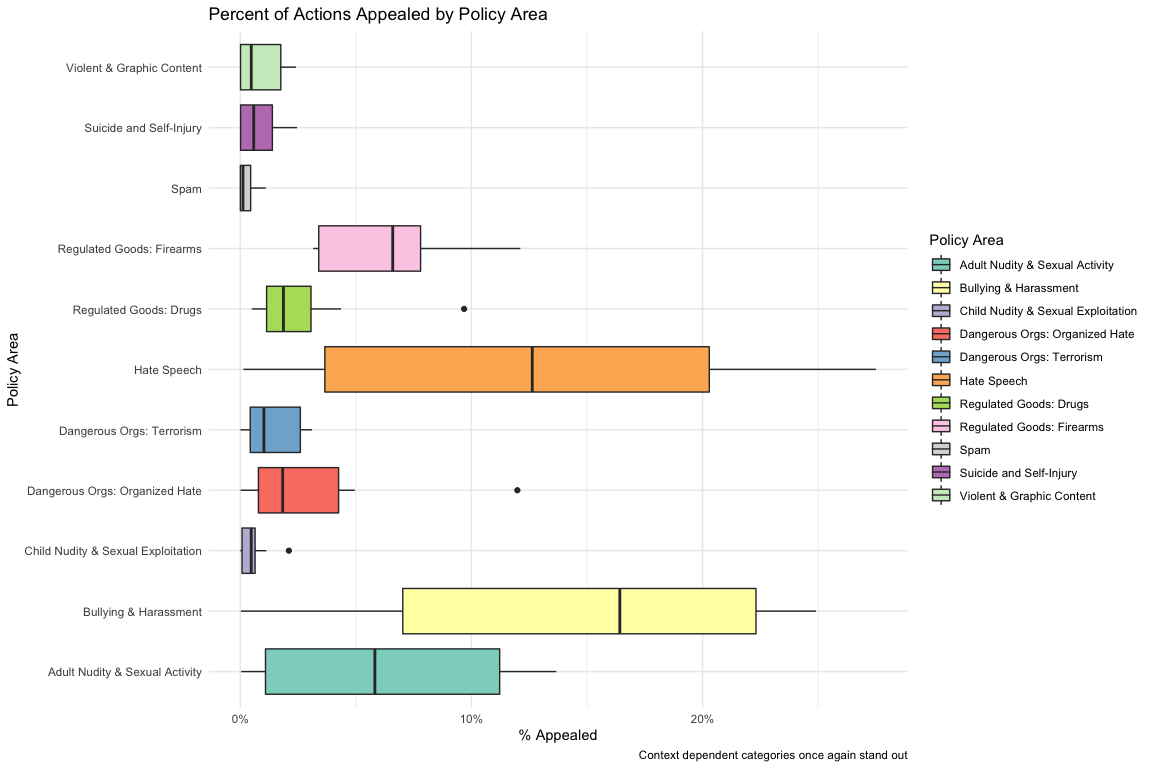
\includegraphics{pdf_document_files/figure-latex/percent appealed box plot-1.pdf}

Indeed, the hypothesis's prediction once again proves accurate. The
percentage of actions against context-dependent content, particularly
Hate Speech and Bullying \& Harassment, is much higher and more variable
than the their more objective counterparts. Interestingly, content
removed for Adult Nudity \& Sexual Activity also appears prone to
appeal. Spam content and Child Nudity \& Sexual Exploitation by
comparison rarely see appeals. Once more the data exposes the errors
made by machine learning algorithms when they flag context-dependent
content.

\hypertarget{conclusion}{%
\section{Conclusion}\label{conclusion}}

\begin{center}\rule{0.5\linewidth}{0.5pt}\end{center}

We conclude by answering my last question. It has become clear from the
analysis above that there are real issues with Facebook's content
moderation system as well the public's understanding of it. Firstly,
while the public focuses on issues like disinformation and hate speech,
Facebook's content moderation is not geared toward nor effective at
resolving these issues. In spite of a recent increase in the number of
actions against Hate Speech, moderation the vast majority of the time
removes less controversial content like spam and fake accounts.

And when the machine learning elements of content moderation do focus on
more objectionable content, they are often ineffective. From hate speech
to disinformation this content is usually only identifiable by
referencing context, which is a challenging task for today's machine
learning algorithms. Advocates of reform to Section 230 must have these
hard realities in mind. The fundamental limits of technology make
incentivizing more aggressive moderation by exposing technology
companies to liabilities for user-generated content a blunt tool to
address the blight of objectionable content.

\hypertarget{session-info}{%
\section{Session Info}\label{session-info}}

\begin{verbatim}
## - Session info ---------------------------------------------------------------
##  setting  value                       
##  version  R version 4.1.0 (2021-05-18)
##  os       macOS Big Sur 10.16         
##  system   x86_64, darwin17.0          
##  ui       X11                         
##  language (EN)                        
##  collate  en_US.UTF-8                 
##  ctype    en_US.UTF-8                 
##  tz       Europe/London               
##  date     2021-09-27                  
## 
## - Packages -------------------------------------------------------------------
##  package      * version date       lib source        
##  assertthat     0.2.1   2019-03-21 [1] CRAN (R 4.1.0)
##  backports      1.2.1   2020-12-09 [1] CRAN (R 4.1.0)
##  broom          0.7.8   2021-06-24 [1] CRAN (R 4.1.0)
##  cachem         1.0.5   2021-05-15 [1] CRAN (R 4.1.0)
##  callr          3.7.0   2021-04-20 [1] CRAN (R 4.1.0)
##  cellranger     1.1.0   2016-07-27 [1] CRAN (R 4.1.0)
##  cli            3.0.0   2021-06-30 [1] CRAN (R 4.1.0)
##  colorspace     2.0-2   2021-06-24 [1] CRAN (R 4.1.0)
##  crayon         1.4.1   2021-02-08 [1] CRAN (R 4.1.0)
##  DBI            1.1.1   2021-01-15 [1] CRAN (R 4.1.0)
##  dbplyr         2.1.1   2021-04-06 [1] CRAN (R 4.1.0)
##  desc           1.3.0   2021-03-05 [1] CRAN (R 4.1.0)
##  devtools       2.4.2   2021-06-07 [1] CRAN (R 4.1.0)
##  digest         0.6.27  2020-10-24 [1] CRAN (R 4.1.0)
##  dplyr        * 1.0.7   2021-06-18 [1] CRAN (R 4.1.0)
##  ellipsis       0.3.2   2021-04-29 [1] CRAN (R 4.1.0)
##  evaluate       0.14    2019-05-28 [1] CRAN (R 4.1.0)
##  fansi          0.5.0   2021-05-25 [1] CRAN (R 4.1.0)
##  farver         2.1.0   2021-02-28 [1] CRAN (R 4.1.0)
##  fastmap        1.1.0   2021-01-25 [1] CRAN (R 4.1.0)
##  forcats      * 0.5.1   2021-01-27 [1] CRAN (R 4.1.0)
##  fs             1.5.0   2020-07-31 [1] CRAN (R 4.1.0)
##  generics       0.1.0   2020-10-31 [1] CRAN (R 4.1.0)
##  ggplot2      * 3.3.5   2021-06-25 [1] CRAN (R 4.1.0)
##  glue           1.4.2   2020-08-27 [1] CRAN (R 4.1.0)
##  gtable         0.3.0   2019-03-25 [1] CRAN (R 4.1.0)
##  haven          2.4.1   2021-04-23 [1] CRAN (R 4.1.0)
##  here         * 1.0.1   2020-12-13 [1] CRAN (R 4.1.0)
##  highr          0.9     2021-04-16 [1] CRAN (R 4.1.0)
##  hms            1.1.0   2021-05-17 [1] CRAN (R 4.1.0)
##  htmltools      0.5.1.1 2021-01-22 [1] CRAN (R 4.1.0)
##  httr           1.4.2   2020-07-20 [1] CRAN (R 4.1.0)
##  jsonlite       1.7.2   2020-12-09 [1] CRAN (R 4.1.0)
##  knitr        * 1.33    2021-04-24 [1] CRAN (R 4.1.0)
##  labeling       0.4.2   2020-10-20 [1] CRAN (R 4.1.0)
##  lifecycle      1.0.0   2021-02-15 [1] CRAN (R 4.1.0)
##  lubridate      1.7.10  2021-02-26 [1] CRAN (R 4.1.0)
##  magrittr       2.0.1   2020-11-17 [1] CRAN (R 4.1.0)
##  memoise        2.0.0   2021-01-26 [1] CRAN (R 4.1.0)
##  modelr         0.1.8   2020-05-19 [1] CRAN (R 4.1.0)
##  munsell        0.5.0   2018-06-12 [1] CRAN (R 4.1.0)
##  pillar         1.6.1   2021-05-16 [1] CRAN (R 4.1.0)
##  pkgbuild       1.2.0   2020-12-15 [1] CRAN (R 4.1.0)
##  pkgconfig      2.0.3   2019-09-22 [1] CRAN (R 4.1.0)
##  pkgload        1.2.1   2021-04-06 [1] CRAN (R 4.1.0)
##  prettyunits    1.1.1   2020-01-24 [1] CRAN (R 4.1.0)
##  processx       3.5.2   2021-04-30 [1] CRAN (R 4.1.0)
##  ps             1.6.0   2021-02-28 [1] CRAN (R 4.1.0)
##  purrr        * 0.3.4   2020-04-17 [1] CRAN (R 4.1.0)
##  R6             2.5.0   2020-10-28 [1] CRAN (R 4.1.0)
##  RColorBrewer * 1.1-2   2014-12-07 [1] CRAN (R 4.1.0)
##  Rcpp           1.0.7   2021-07-07 [1] CRAN (R 4.1.0)
##  readr        * 1.4.0   2020-10-05 [1] CRAN (R 4.1.0)
##  readxl         1.3.1   2019-03-13 [1] CRAN (R 4.1.0)
##  remotes        2.4.0   2021-06-02 [1] CRAN (R 4.1.0)
##  reprex         2.0.0   2021-04-02 [1] CRAN (R 4.1.0)
##  rlang          0.4.11  2021-04-30 [1] CRAN (R 4.1.0)
##  rmarkdown      2.9     2021-06-15 [1] CRAN (R 4.1.0)
##  rprojroot      2.0.2   2020-11-15 [1] CRAN (R 4.1.0)
##  rstudioapi     0.13    2020-11-12 [1] CRAN (R 4.1.0)
##  rvest          1.0.1   2021-07-26 [1] CRAN (R 4.1.0)
##  scales         1.1.1   2020-05-11 [1] CRAN (R 4.1.0)
##  sessioninfo    1.1.1   2018-11-05 [1] CRAN (R 4.1.0)
##  stringi        1.6.2   2021-05-17 [1] CRAN (R 4.1.0)
##  stringr      * 1.4.0   2019-02-10 [1] CRAN (R 4.1.0)
##  testthat       3.0.4   2021-07-01 [1] CRAN (R 4.1.0)
##  tibble       * 3.1.2   2021-05-16 [1] CRAN (R 4.1.0)
##  tidyr        * 1.1.3   2021-03-03 [1] CRAN (R 4.1.0)
##  tidyselect     1.1.1   2021-04-30 [1] CRAN (R 4.1.0)
##  tidyverse    * 1.3.1   2021-04-15 [1] CRAN (R 4.1.0)
##  usethis        2.0.1   2021-02-10 [1] CRAN (R 4.1.0)
##  utf8           1.2.1   2021-03-12 [1] CRAN (R 4.1.0)
##  vctrs          0.3.8   2021-04-29 [1] CRAN (R 4.1.0)
##  withr          2.4.2   2021-04-18 [1] CRAN (R 4.1.0)
##  xfun           0.24    2021-06-15 [1] CRAN (R 4.1.0)
##  xml2           1.3.2   2020-04-23 [1] CRAN (R 4.1.0)
##  yaml           2.2.1   2020-02-01 [1] CRAN (R 4.1.0)
## 
## [1] /Library/Frameworks/R.framework/Versions/4.1/Resources/library
\end{verbatim}

\end{document}
